%%%% fs-run-mapreduce Optimistic collision management
\label {fs-collision}

As it was defined previously, only the grouping operation maintains a state and the state depends on the order of incoming items. Because of asynchrony and the possible existence of multiple paths between two nodes it is hard to deliver the right order.

In order to address this issue, we accept the fact that grouping can produce incorrect tuples. However, we guarantee that all correct tuples are eventually produced. The correctness of tuple means that this tuple would be generated if the order assumption was satisfied. 

To eventually produce all correct tuples, we use an approach called {\it replay}. If an item arrives the grouping operation, according to the meta-information order, nothing is replayed and only the most recent window is produced. However, if an item is out-of-order, it is inserted in the bucket at the correct location, and all tuples, which contain this element, are reproduced. Thereby, replay guarantees that eventually all correct tuples are generated. At the same time, for tuples, that has been produced but became invalid, {\it tombstones} are sent.

Tombstones are ordinal data items but with a special flag in its meta-information. This flag means that tuples with such meta-information are invalid, and they should not leave the system. Tombstones have the same payloads as invalid items in order to go through the same path in the computational pipeline.

The example of replay is shown in Figure~\ref{grouping-replaying}, The green item is out-of-order. The ouput consists of the new valid items, {\it (1, 2) and (2, 3)}, and the tombsone, {\it (1, 3)}.

\begin{figure}[htbp]
  \centering
  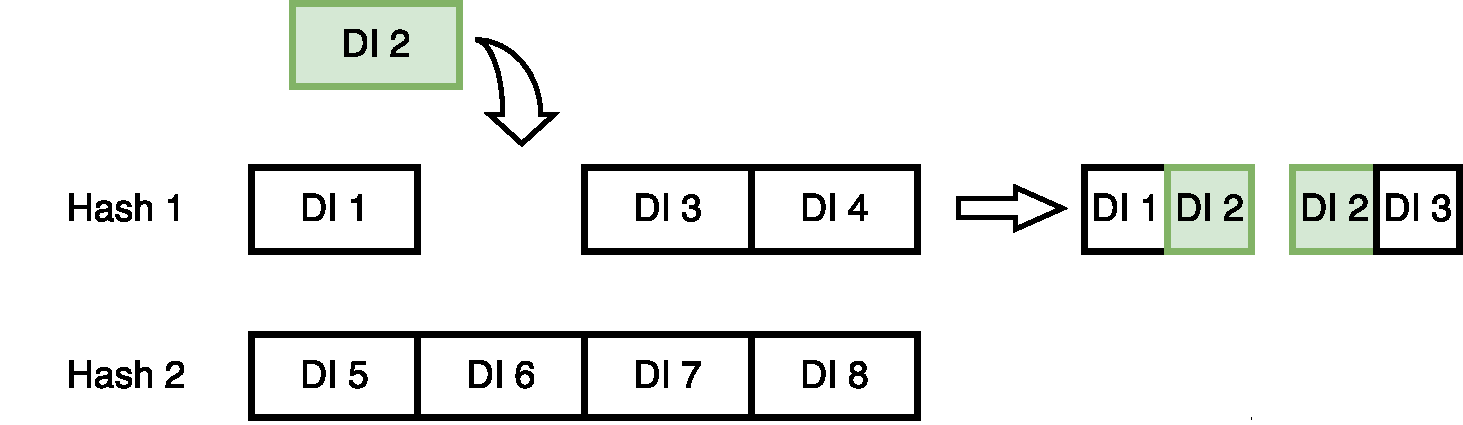
\includegraphics[width=0.48\textwidth]{pics/grouping-replaying}
  \caption{The replay in groupig with window = 2. The new items are generated on insertion}
  \label {grouping-replaying}
\end{figure}

In the case of the right order of input items, there are no redundant items produced.

The barrier filters out invalid elements, when corresponding tombstones arrive. It is partially flushed for some meta-information interval when there is a guarantee that there are no any out-of-order items and tombstones further up the stream for this range. The exact technique for providing such guarantee is defined further.

\subsubsection{Meta information}
The meta-information of data item is a tuple of a {\it global time}, a {\it trace}, {\it child ids} and a tombstone flag.

\[Meta := (GlobalTime, ChildIds[], Trace, IsTombstone)\]

Global time is assigned to data item once the item enters the system. It is a pair of milliseconds since the epoch start and the identifier of the front. The identifier is used to assign different global times to different items, even in case of wall-clock collisions. 

\[GlobalTime := (FrontTs, FrontId)\]

Global times are compared by front timestamp if they coincide - by front id. It is important to notice, that we are not relying on any clock synchronization between nodes, but we require a strict monotonicity within the single front. The only implication of the clock skew is the system degradation in terms of latency: 1ms of the nodes clock difference appends 1 ms to minimal latency.

Each map operation can produce multiple items from one. To differentiate them the ordinal number, {\it child id}, is stored in the meta information. The {\it ChildIds } is an array of child ids, that corresponds to the all visited map operations.

The global time and child ids are enough to uniquely identify data item within stream, if all processing is done without replays. If there are any replays happened during processing, multiple items with the same global time and child ids exist in the stream. Multiple tombstones with the same global time and child ids can exist as well. They can take different paths in computational flow and travel within them with different speeds. 

Despite this fact, an invalid element and the corresponding tombstone are go through the same path, because they have the same payload and the balancing functions are deterministic. Moreover, the tombstone visits operations strictly after corresponding item, as links between operation are expected to be FIFO. 

To match tombstone with proper item there is {\it Trace} value stored in the meta-information. Trace encodes the path item have traversed. Each phsical copy of each operation is assigned with unique random 64-bit identifier. The trace is a xor of the all operations' ids visited by item so far.

\[Trace := \bigoplus_{op \in \text{visited}} Id(op)\]

Metas are compared lexicographically: firstly global times are compared, then child ids, then traces. Notably, this order is in line with the \FlameStream's ordering model.

Figure~\ref{logical-graph-ops-figure} shows the topology of each operation and how it affects the meta. Grouping and merge operations update trace of data item by xoring initial trace with its physical id. Map and broadcast apply the same update, but also append child id for each output item.

\begin{figure}[htbp]
  \centering
  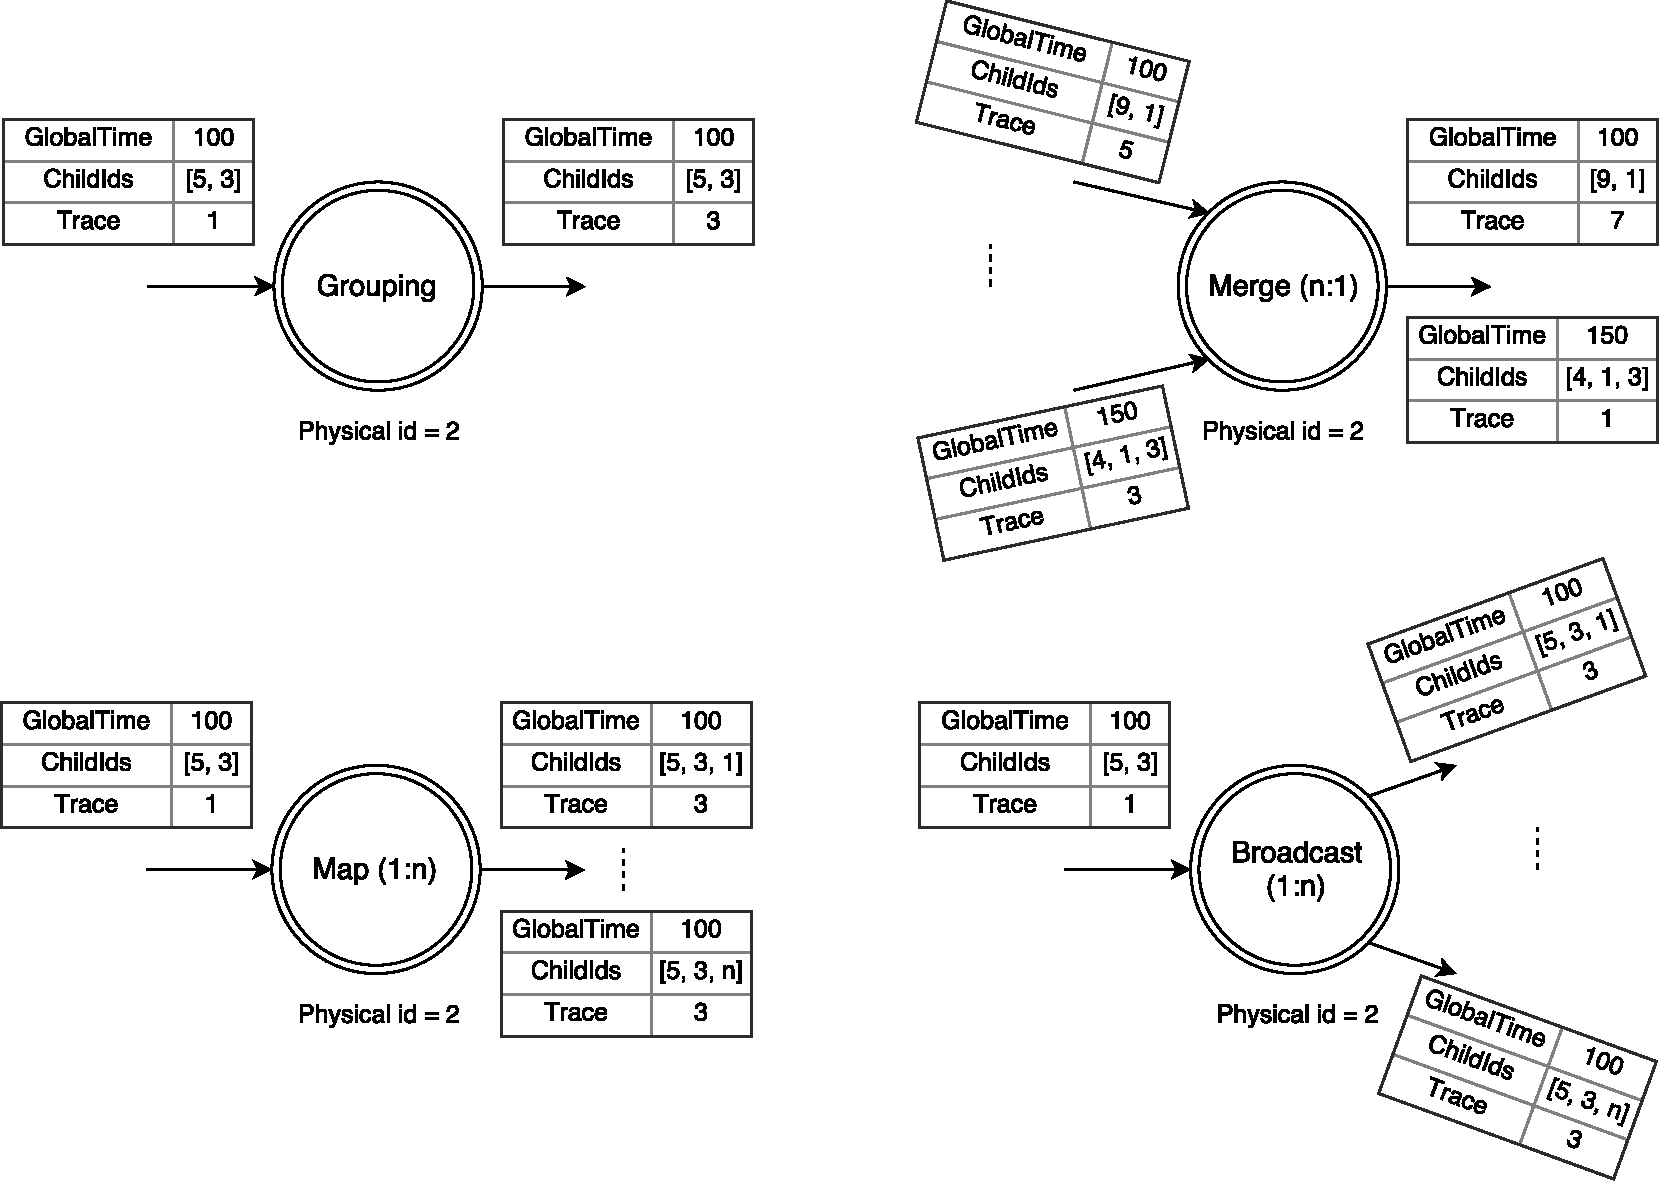
\includegraphics[scale=0.5]{pics/operations}
  \caption{Meta-information handling}
  \label {logical-graph-ops-figure}
\end{figure}

The structure of meta provides for tracking different relations between data items:

\begin{itemize}
  \item Items with same global time and common prefixes are produced from the same item
  \item Item with lower meta is generated earlier, at front or in the stream
  \item If there are two items with the same global time and child ids, only one of them is the right one
\end{itemize}

\label{mininal-time}
\subsection{Minimal time within stream}

To release the item from the barrier we need to ensure that there are no in-flight tombstones. 

\newtheorem{minimal-time-claim}{Lemma}

\begin{minimal-time-claim}
  If data item {\it D} has global time {\it GT} greater than the global time of the in-flight elements, then all tombstones for that item had already arrived at the barrier.
\end{minimal-time-claim}

\begin{proof}
  Let $D_{tomb}$ is in-flight tombstone for {\it D}. According to the definition of the tombstone item, $D_{tomb}$ and {\it D} has the same global time {\it GT}. We assumed that there are no in-flight element with the global time equal to {\it GT}. Contradiction.
  
  It is worth to note, that new tombstones for {\it D} cannot be generated, because items with global time greater than {\it GT} cannot trigger replay that affects {\it D}.

  This implies that if the stream does not contain items with the global time less than or equal to {\it GT}, then all tombstones for {\it D} had already arrived at the barrier. 
\end{proof}

Therefore, to output an item from the barrier, we should ensure that there are no items in the stream with the global time less than or equal to the global time of this item.

To track the global time of in-flight items we adopt an idea of {\it acker task} inspired by Apache Storm~\cite{apache:storm}. Acker tracks data items using a checksum hash. When the item is sent or received by an operation, its global time and checksum are sent to the acker. This message is called {\it ack}. Acker groups acks by a global time into the structure called {\it ack table}. Once acker receives an ack message with global time {\it GT} and {\it XOR} it updates {\it GT} entry in the table by xoring {\it XOR} with the current value. When an item is sent and later received by the next operation, xoring corresponding {\it XOR}s would yield zero.

Acks are overlapped to nullify table's entry only when an item arrives at the barrier. That is, ack for receive is sent only after both processing and the ack sending for the transformed item, as illustrated in Figure~\ref{acker}. Different shapes of items mean different payloads. The ack for the sending of the triangular element is sent before the rectangular one. We expect the channel between the acker and each operation to be FIFO, so ack for the triangular item would be xored before the rectangular. So the two equal values are separated by distinct one. 

This technique guarantees that the {\it XOR} for some global time is equal to zero only if there are no in-flight elements with such global time.

\begin{figure}[htbp]
  \centering
  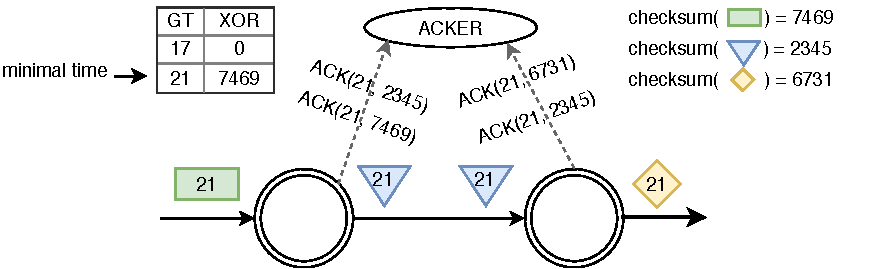
\includegraphics[scale=0.5]{pics/acker}
  \caption{Acker}
  \label {acker}
\end{figure}

The minimal time within a stream is the minimal global time with non-zero {\it XOR}. On minimal time changes, acker broadcasts new minimal time to the barrier and operations. Therefore, the barrier can release elements with global time {\it GT} once it received notification from acker that the minimal time within the stream is greater than {\it GT}.

To ensure that no fronts are able to generate item with the certain timestamp, each front periodically sends to acker special message called {\it report}, which promises that front will not generate items with a timestamp lower than the reported. The value in the ack table can become a zero only after the corresponding report arrives.

The proposed mechanism could be isolated by hash range. This change allows us releasing from barrier independent also known as early key availability.
